% Chapter 1

\chapter{Introduction} % Chapter title

\label{ch:introduction} % For referencing the chapter elsewhere, use \autoref{ch:introduction} 

\begin{flushright}{\slshape    
Multimedia is not more media, \\ 
but the employment of various kinds of media (and hybrid media) \\ 
for what they each offer to advance the narrative.} \\ \medskip
--- \defcitealias{ritchin:2013}{Fred Ritchin}\citetalias{ritchin:2013} \citep{ritchin:2013}
\end{flushright}

\section{Challenges of Multimedia}
The main subject of this dissertation is \textbf{multimedia}, content that combines multiple forms of media such as text, graphics, audio and video. In particular, we focus on \textbf{audiovisual media} that have both a sound and a visual component. For example, presentations that involve graphics and sound, audiobooks that combine text with audio, and videos that incorporate graphics, sound and text are all different types of audiovisual media. \\

As these everyday examples illustrate, audiovisual media has become commonplace. From the consumer's perspective, we encounter them in our normal activities, for instance, listening to a podcast, watching an advertisement or sitting in on a presentation. We also frequently produce audiovisuals to communicate our ideas, for example, by creating a blog or sharing a video on YouTube. In addition, new technologies and online platforms encourage new types of audiovisual media such as GoPro videos, 360-degree videos, interactive infographics or online lectures.\\ 

Unfortunately, ease of access does not translate directly to efficiency or good quality. Simply navigating audiovisual media to search for information can be tedious. Consider the times you had to listen to a voicemail repeatedly to get the call back number, or when you had to play the video back and forth to find a specific moment. Producing compelling audiovisual media is even more time-consuming and difficult. People spend hours to produce a single slide of presentation or a few seconds of video.\\ 

A major part of the difficulty lies in the nature of multimedia itself. For one, as its name implies, multimedia blend multiple modalities, each of which have different characteristic strengths and weaknesses. Let's consider some of the basic components of multimedia.
\begin{description}
\item[Text:] As a static representation of language, text is one of the most common forms of communication that most people are familiar with. It is easy to author and edit digitally, and many algorithms exist to process text, for instance, for text summarization or comparison. Text is also easy to navigate by skimming or searching. It can be organized spatially to emphasize structure and further facilitate navigation. In addition, different visual attributes such as typeface, font size or color can be used to convey extra information such as emphasis.\\
On the other hand, some types of information is less suited for textual representation. For example, describing a complicated diagram or a piece of music would be difficult to achieve using text alone. There is also a limit to conveying tonal nuances or voice. \\

%
\marginpar{
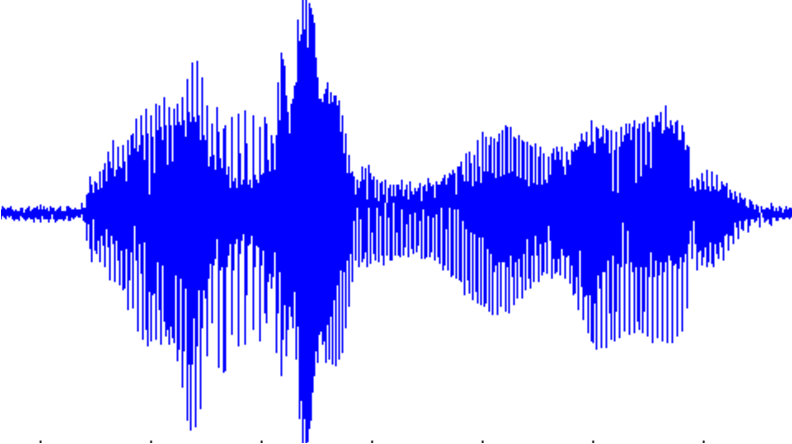
\includegraphics[width=1.2in]{figures/waveform.pdf}
\captionsetup{font=footnotesize}
 \captionof{figure}{Audio represented in waveform. }
\label{fig:waveform}
}
%
\item[Audio:] Audio is a rich source of information that can convey not only speech but any other sound that may not have an accurate textual description, for example, the sound of a heartbeat or the sound of waves. It is an effective media for evoking emotion or reflecting mood.\\
However, most audio lack appropriate visual representation, which makes it difficult to navigate or edit. Waveform is the most generic representation used in many applications, but it is ambiguous and hard to manipulate (Figure~\ref{fig:waveform}). 
For instance, detecting or separating the sound of one instrument from a music recording is a challenging research problem.\\

\item[Image:] A picture is worth a thousand words. Human perception is visually oriented, so images can be a powerful tool to communicate rich information intuitively in a small amount of space. Images are especially useful for conveying spatial relationships, structure, or detailed shape. Consider describing the layout of a building or the features of a face only using words versus showing a picture of the floor plan or the face.\\ 
On the other hand, it is difficult to convey information about movement or sequence using a still image. Oftentimes, text, labels or animation effects are attached to a still image to focus the viewers' attention to a specific part of the image or to clarify the intended message.\\

\item[Animation/Video:] Animations are created from a set of static frames whereas videos record a continuous event which is then broken up into a series of frames. Both media are especially useful for illustrating concepts that involve motion or sequence.\\
As with audio, it takes time to navigate through the content of an animation or video and it is difficult to skim or search.\\

\item[Time:] In addition to having multiple modalities, audiovisual media is also intricately linked with time. Time imposes a linear structure to the media and is expressed, for example, with timelines on videos, scrollbars on websites and page numbers on slides. Whereas time provides a natural order to the media, it can also make non-linear interactions more cumbersome. For instance, watching a video from beginning to end is easy, but searching for specific scenes is harder.\\
Time also imposes a certain speed or pace to the media, and makes each \textit{moment}  within the media transient. Video frames, parts of webpages or slides are displayed for a limited amount of time and replaced with different, successive information. The abundance of concurrent and transitory information makes audiovisual media difficult to digest and manipulate compared to static media.\\
Finally, synchronization between multiple modalities is an essential part of audiovisual media. Effective navigation and manipulation of the media both require that the concurrence between multiple modes is appreciated and maintained. For instance, editing the audio track of a video normally requires editing the corresponding visual footage as well.
\end{description}

In sum, the complex interplay of multimodal information with each other and with time makes audiovisual media difficult to author, edit or navigate efficiently. Workflows around audiovisual media usually involve nonlinear navigation and iteration between different modalities. Unfortunately, conventional media browsers are best suited for linear navigation. Prevalent editing tools also handle each modality independently, leaving users to manage their interconnection manually. Both consumers and producers of audiovisual media have a right to be frustrated at the inefficiency caused by the lack of \emph{user-friendly} and \emph{media-friendly} interfaces that takes into account the users' workflows and characteristics of the media.\\ 
%
\section{The Goal: Effective Interfaces for Multimedia}
Just as effective multimedia carefully blends different types of media to advance the narrative, effective \textit{interfaces} for multimedia must capitalize the characteristics of each medium to expose the media to the users and provide tools to interact with it efficiently. Well-designed interfaces facilitate the users' workflow, be it authoring, editing or browsing, and whether it is linear or nonlinear. With the help of such interfaces, working with audiovisual media should be as simple and natural as working with text documents.\\

Text documents are easy to navigate. One can read it carefully or skim through it. There are efficient techniques to search for specific information. For example, table of contents, index, alphabetically organized dictionaries and simple text search functions are well-established systems that are easy to use. Similarly, we create and edit text documents everyday seemingly effortlessly, whenever we write an e-mail, a business report or a letter.\\

As natural as it seems today, text documents did not start out as an easy medium.
% 
\marginpar{
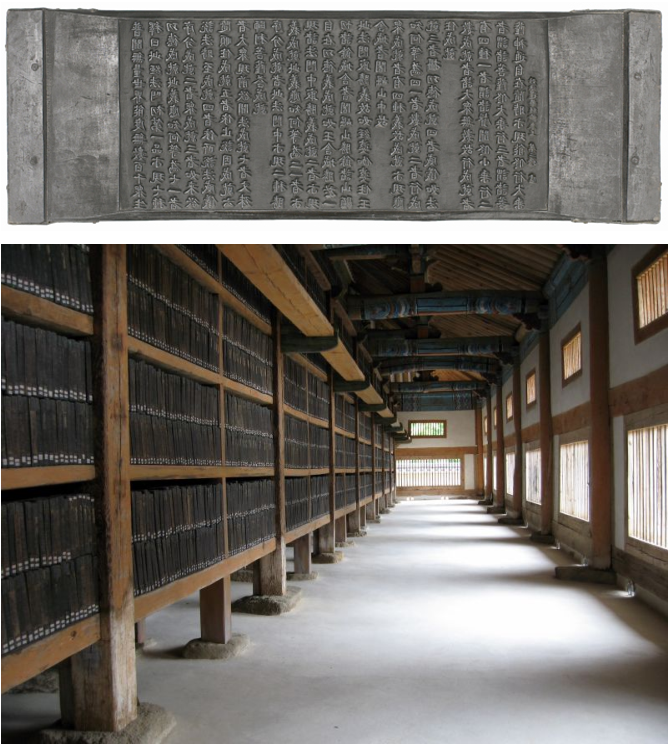
\includegraphics[width=1.2in]{figures/tripitaka_koreana.pdf}
\captionsetup{font=footnotesize}
 \captionof{figure}{Before convenient interfaces were developed, text documents were neither easy to author nor simple to navigate. Tripitaka Koreana, a collection of Buddhist scriptures carved onto 81,258 wooden printing blocks in 13th century Korea. (Above) Each wood block measures 24cm x 70cm. (Below) The blocks are stored in Haeinsa, a Buddhist temple in South Korea.}
\label{fig:tripitaka}
}
%
Consider the 16-feet long scroll containing the text of the Diamond Sutra printed in 9th century China, or the Tripitaka Koreana, a collection of Buddhist scriptures carved onto 81,258 wooden printing blocks in 13th century Korea (Figure~\ref{fig:tripitaka}). These text documents were neither painless to author nor easy to navigate. Even after the advent of digital word processors in the 1960s, it took several decades until the \emph{what-you-see-is-what-you-get} (WYSIWYG) form of word processors as we know them today became commonplace. Now, with online applications such as Google Docs, users can even collaborate on a single text document synchronously or asynchronously with ease. Wikipedia is an example of a new type of collaborative document that became possible through the development of online, collaborative text editors. \\

Similar to text documents, better interfaces can make it easier for users to author, edit, navigate and collaborate on audiovisual media. Improved efficiency can also lead to greater expressivity and even new types of media. This dissertation takes a step towards this goal by exploring several approaches to designing effective interfaces for audiovisual media.

\section{Opportunities for Multimedia Interfaces}
Previously, we demonstrated that the complex combination of multiple modalities make multimedia especially difficult to navigate and manipulate. Yet, the same multimodal quality can be turned into opportunities for designing effective user interfaces for multimedia. The specific design strategy of an interface depends on the media as well as the interaction that the interface is trying to support (e.g., authoring, editing or browsing). Here, we outline several broad principles that emerged through our work on several different applications.\\
%

\subsubsection*{Principle 1. Harness spatial and temporal structure:}
The different components of multimedia are tightly associated with each other in time and space. For instance, video frames that are adjacent in time are likely to have similar content. Simultaneous audio and visuals are also closely related to each other. Even within a single image or a slide, spatial layout can reveal meaningful patterns about the content.\\

Inferring the spatial and temporal structure embedded in the media can help design effective interactions. For one, explicitly visualizing the structure can help viewers navigate the media efficiently. In addition, interfaces can facilitate editing by keeping track of and maintaining meaningful structure, for instance, the synchronization between different components. \\

\subsubsection*{Principle 2. Exploit different modalities to facilitate various types of interaction:}
Each modality that compose audiovisual media lends itself more naturally to different types of user interaction or user tasks. For example, during navigation, text is easier to skim or search, whereas audio is more effective in conveying tonal nuances or flow. During authoring, speaking is faster than writing, but editing audio is generally more time consuming than editing text.\\

Interfaces for audiovisual media can take advantage of different modalities or representations to facilitate different parts of user tasks. For example, in Chapter~\ref{ch:voicescript}, we propose an interface for authoring voice recordings, which supports both authoring via speech and editing via text.  A key challenge in designing such multimodal interfaces is to enable seamless interaction between the different modalities. That is, edits in one modality should be translatable into meaningful operations in other modalities.\\  

\subsubsection*{Principle 3. Support direct manipulation with automation:}
Hybrid approaches that combine direct manipulation with automatic algorithms have been proposed and successfully implemented in many application domains, including authoring of 3D models \cite{gal2009iwires, prevost2013make}, animations \cite{bai2016artist}, and illustrations \cite{chi2012mixt}. Automatic algorithms can greatly simplify tedious tasks and allow users to focus on the creative part of the workflow.\\

In light of the previous two principles, automatic algorithms can also take advantage of the inherent structure of the media or characteristics of different modalities. For example, in Chapter~\ref{ch:visualtranscript}, we use an automatic algorithm to extract  a set of static images from a video by analyzing the spatial and temporal structure of the visuals drawn continuously in the video. In Chapter~\ref{ch:voicescript}, we take advantage of text--a discrete modality that is easier to process automatically--in order to compare and align audio. Finally, in Chapter~\ref{ch:aparecium}, we use pre-authored digital slides to achieve, among other things, real-time beautification effects of hand-drawn strokes.\\ 

As the following chapters will illustrate, these principles are instantiated for each application through a combination of interface design, visualization, algorithms and data structures.

%----------------------------------------------------------------------------------------
\section{Overview}
This dissertation is about designing effective interfaces to support the authoring and navigation of multimedia. We explore a range of applications -- navigating lecture videos, authoring speech recordings and delivering slide presentations. We originally considered these applications in separate publications, presented to different communities in computer graphics and human computer interaction. The goal of this text is to distill the common theme across these applications and present them in a unified way, along with insights gained over the course of our work. Subsequent chapters are organized by application domain:\\


\subsubsection*{Navigating Lecture Videos (Chapter ~\ref{ch:visualtranscript}):}
Lecture videos are widely used for learning, but existing
video player interfaces are poorly equipped to support frequent learner tasks. For example, it is difficult to search or skim the content, or view the lecture material at one's own pace. For these and other reasons, some people prefer to read lecture notes than to watch videos.\\

To facilitate learning with videos, we propose \textbf{VisualTranscript}, a readable and skimmable interface for lecture videos. VisualTranscript transforms blackboard-style lecture videos into interactive lecture notes, interleaving static figures with hierarchically organized paragraphs of text.\\

We describe automatic algorithms to (1) extract a discrete set of key illustrations from the video frames, and (2) to analyze the audio content and classify sentences into two categorizes: depictive sentences that verbalize what the illustrations depict, and explanatory sentences that provide additional information not directly represented by the illustrations. Both algorithms take advantage of spatial and temporal structures inferred from the video.\\

We compare VisualTranscript with a standard video player, and a state-of-the-art interface designed specifically for blackboard-style lecture videos. User evaluation suggests
that users prefer VisualTranscript for learning and that VisualTranscript is
effective in helping them browse or search through lecture videos.\\

\subsubsection*{Authoring Speech Recordings (Chapter~\ref{ch:voicescript}):}
Speech recordings are central to modern media from podcasts
to audio books to e-lectures and voice-overs. Authoring these
recordings involves an iterative back-and-forth process between
script writing/editing and audio recording/editing. Unfortunately, most
existing tools treat the script and the audio separately, making
the iterative workflow very tedious.\\

We present \textbf{VoiceScript}, an interface to support a dynamic workflow for script
writing, audio recording and audio editing. VoiceScript integrates the
script with the audio such that, as the user writes the script or
records speech, edits to the script are translated to the audio
and vice versa.\\

Through informal user studies, we demonstrate that VoiceScript greatly facilitates the audio authoring process in various scenarios.\\

\subsubsection*{Delivering Slide Presentations(Chapter~\ref{ch:aparecium}):}
Presentations are an important component of both classroom
and online instruction, and presentation tools have a significant impact on how we teach and learn. Electronic slides, the dominant type of presentation technology today, has several shortcomings. Pre-authored slides take long time to prepare and restrict how contents are presented. There is little flexibility on the order and granularity of how information is displayed during the presentation.\\

We introduce \textbf{Aparecium}, a presentation interface that helps presenters deliver flexible and engaging presentations by combining
the aesthetics and organization of electronic slides with
the spontaneity of inking. In Aparecium, presenters use inking
interactions to deliver slide presentations. With inking, presenters
can (1) reveal pre-authored content to the audience,
(2) make annotations on top of the slide, and (3) adjust the
slide layout to create blank space. Pre-authored slides help improve
the visual aesthetics and organization of the slides, while
inking enables presenters to have flexibility and fine-grained
control over the content and pace of the presentation.\\

In a user study comparing Aparecium with baseline presentation
tools, we found that our interface generally improves presentation
quality without increasing the burden on the presenter
at authoring or presentation time. Especially for text-centered
or process-driven content, both audiences and presenters preferred
presentations delivered using Aparecium.\\

\subsubsection*{}
Finally, Chapter~\ref{ch:conclusion} reviews our contributions and discusses insights gained from our work. The remainder of this chapter offers a brief overview of related work on multimedia interfaces.  
%----------------------------------------------------------------------------------------

\section{Related Work}
\label{main-relatedwork}
Not surprisingly, \textbf{interfaces for multimedia} is a very broad subject that touches many fields of research, including human-computer interaction, computer vision, and computer graphics. Instead of attempting to compile a comprehensive summary of the subject, we broadly categorize previous research according to different phases of users' workflows--browsing, authoring and delivery--and briefly review work that is closely related to the applications we present in this dissertation. The works cited are not intended to be an exhaustive list, but rather serves as an illustrative guide to various topics.

\subsection{Browsing}
A main purpose of media browsing interfaces is to improve the users' efficiency by making it easier to find and absorb useful information--in short, to reduce the browsing time. Although specific techniques vary by media type and content, there are common strategies that apply across different media. \\

\subsubsection*{Displaying Compact Visual Representation:}
Skimming and browsing are inherently visual tasks, and we perform them instinctively, for example, while we read or window-shop. Compact visual representations of media can facilitate navigation by taking advantage of our natural visual capacity. \\

Visual abstratctions of a video can take many forms such as shorter video skims ~\cite{chu2015video,lu2013story}, keyframes~\cite{kim2014joint,khosla2013large}, montages~\cite{sun2014salient}, collages~\cite{wang2007video} and panoramas~\cite{liu2008discovering,choudary2007summarization}. It can combine static images or videos with text~\cite{papernick2005summarization}. Static representations can also take advantage of spatial layout to expose the structure of the video. For example, Boreczky et al. arrange selected keyframes into a comic style layout, representing important segments with larger frames~\cite{boreczky2000interactive} . Interactive techniques can enhance the summary, for example by allowing users to explore the video by zooming in to expose fine-scale temporal details~\cite{barnes2010video}.\\

Unlike video, audio is a medium that does not have a natural visual representation. Nevertheless, from early on graphical representations have been used to facilitate visual scanning and searching of audio, and in particular, speech~\cite{schmandt1981intelligent,degen1992working}. It has been shown that transcript texts are highly effective as an interface to support browsing~\cite{schmandt1981intelligent,whittaker1999scan}. In some applications, accompanying visual media such as handwritten notes~\cite{whittaker1994filochat,stifelman2001audio} or video~\cite{kazman1996four,hauptmann1997informedia} are also used to index audio.\\ 

\subsubsection*{Analyzing and Exposing Structure within Media:}
In order to construct an effective visual representation, it is usually necessary to infer some type of structure from the media. For example, videos are summarized by extracting highlight scenes~\cite{chen2011formulating,fleischman2007temporal}, topical themes~\cite{wu2006threading}, or repetitive segments~\cite{Chu_2015_CVPR,Zhao_2014_CVPR}. Similarly, speech browsing interfaces take advantage of inferred speaker turns~\cite{wilcox1994segmentation}, emphasis~\cite{arons1994interactively} or pauses~\cite{arons1997speechskimmer}. These information can be inferred from the main modality itself (e.g., extracting repetitive structure in music from its signal~\cite{cooper2003summarizing}), from accompanying modalities (e.g., extracting highlights of baseball games from audio ~\cite{rui2000automatically}), or from additional sources (e.g., using screenplay to infer scene hierarchy of a movie~\cite{cour2008movie,pavel2015sceneskim}). They can be computed automatically~\cite{cooper2003summarizing,rui2000automatically,pavel2015sceneskim} or with the help of manual annotation~\cite{chi2013democut,pavel2014video}.\\

\subsection{Authoring}
\label{sec:relatedwork-authoring}
Authoring covers a wide range of tasks from capturing and browsing the source to drafting and editing the final product. An important objective of authoring interfaces is to make this workflow from the initial source to the final output as fluid as possible. There are many considerations that go into supporting this goal. Here, we consider two themes that arise commonly across applications. 

\subsubsection*{Translating between Modalities:} The modality of the final output is not necessarily the most convenient modality to interact with during the authoring process. Many studies attempt to facilitate authoring by enabling easier, less formal input modalities such as text, pen-interactions or gestures, and translating them into appropriate operations on the final product. For example, transcript texts are used to edit videos~\cite{berthouzoz2012tools,casares2002simplifying} or audio recordings~\cite{rubin2013content}, hand-drawn sketches are translated into informal presentations~\cite{li2003sketching} or website designs~\cite{lin2000denim}, and physical gestures are captured to create cartoons~\cite{nara2013manga} or 3D animations~\cite{held20123d}.\\

The increasing availability of various types of interactive devices is also encouraging research in multimodal interfaces that support a combination of input modalities. For example, MultiPoint uses speech and pen to author presentation slides~\cite{sinha2001multipoint}, while PixelTone combines speech and direct manipulation to edit photos~\cite{laput2013pixeltone}. These interfaces aim to support a more \emph{human} way of interacting with digital media similar to our day-to-day communication methods. Recent survey papers~\cite{turk2014multimodal,dumas2009multimodal} provide a comprehensive review of this subject.\\

\subsubsection*{Analyzing and Exploiting Relationship between Media:} 
It is common to combine multiple raw sources (e.g., video footage, audio tracks) to compose a single output media. Similar to browsing that takes advantage of inherent structures within a single media, editing can exploit inherent relationships between multiple streams of media. For example, Arev et al. infer the 3D spatial relationship between multiple cameras capturing a social event in order to produce a coherent cut video of the event~\cite{arev2014automatic}. Bryan et al. synchronize multiple-camera videos of a same event using audio features~\cite{bryan2012clustering}. QuickCut facilitates editing of narrated videos by aligning audio narration with semantically relevant video segments by taking advantage of user annotations and the narration transcript~\cite{truong2016quickcut}. Li et al. present a method to synchronize slideshows of paintings to accompanying music by analyzing their common emotional features~\cite{li2007emotion}. Unlike work on video or audio summarization, these work deal with relational structures across multiple input sources. 

\subsection{Delivery}
Once authored, most media is delivered \emph{as-is} to the consumer in a static format. However, some media such as presentations involve a dynamic aspect in which the media can be delivered interactively in a live setting. Improving flexibility for live performance is a key focus in this area.

\subsubsection*{Supporting Flexible Modes of Interaction:} One strategy to improve flexibility during performance is to support flexible modes of interaction to control the media. For example, instead of predetermined linear presentations, Palette provides random access to slides using physical cards~\cite{nelson1999palette}. Similarly, zooming user interfaces allow flexible presentation paths through spatial navigation of slides~\cite{lichtschlag2009fly,good2002zoomable}. Baudel and Beaudouin-Lafon propose hand gestures as an intuitive mode to control slides~\cite{baudel1993charade}. Other work enable presenters to add improvised content by inking~\cite{anderson2007classroom,golub2004handwritten}. A common concern across these work is providing and intuitive interaction mode that does not further burden the presenter at performance time.\\ 

\subsection*{}
Each of our work focuses on a different media and a different part of the users' workflow. However, they are inspired by many of the same principles that we observe in previous work. In each chapter, we also include a review of work that is more directly related to the application being discussed. 
 

